\documentclass[14pt]{extreport}
\usepackage{indentfirst}
\usepackage[T2A]{fontenc}
\usepackage[utf8]{inputenc}
\usepackage[english,russian]{babel}
\usepackage{parskip}
\usepackage[top = 20mm, left = 20mm, right = 20mm, bottom = 20mm]{geometry}
\setlength\parindent{12.5mm} 
\renewcommand{\baselinestretch}{1.5} 
\def\hrf#1{\hbox to#1{\hrulefill}} 
\usepackage{ragged2e} 
\usepackage{caption}
\usepackage{tikz}
\usepackage{circuitikz}
\usetikzlibrary{decorations.pathmorphing,arrows.meta}
\usepackage{multicol}
\usepackage{float}
\usepackage{tipa}
\usepackage{graphicx}
\usepackage{enumitem}
\usepackage{amsmath}
\usepackage{amssymb}
\usepackage{listings}
\usepackage{moreverb}
\usepackage{minted}
\setcounter{tocdepth}{3}
\setcounter{secnumdepth}{3}

\lstset{
    language=C++,
    basicstyle=\ttfamily\footnotesize,
    numbers=left,               % Нумерация строк слева
    numberstyle=\tiny\color{gray}, % Стиль номеров строк
    stepnumber=1,               % Номер на каждой строке
    numbersep=5pt,              % Расстояние от номеров до кода
    breaklines=true,            % Перенос длинных строк
    tabsize=2,                  % Размер табуляции
    extendedchars=false,
    keepspaces=true,
    showstringspaces=false,
    frame=single,               % Рамка вокруг листинга
    captionpos=t,               % Подпись сверху
    xleftmargin=10pt,
    xrightmargin=5pt
}
\usepackage[colorlinks=true, citecolor=blue, urlcolor=blue, linkcolor=blue]{hyperref}
\renewcommand\thesection{\arabic{section}}


\begin{document}

\thispagestyle{empty}
    \centering{
    \hspace{0.2cm}МИНИСТЕРСТВО НАУКИ И ВЫСШЕГО ОБРАЗОВАНИЯ РОССИЙСКОЙ ФЕДЕРАЦИИ\\
    Федеральное государственное автономное образовательное учреждение высшего образования\\
    {\bf «Санкт-Петербургский политехнический университет Петра Великого»}\\[10pt]
    Институт компьютерных наук и кибербезопасности\\
    Высшая школа технологий искусственного интелекта\\
    02.03.01 Математика и компьютерные науки\\
    \vspace{1.5cm}
    {\large
    \bf Отчет\\
    \bf Структуры данных}\\
    {\large\bf Летняя научно-исследовательская работа}\\
    \vspace{\fill}
    }
    \vspace{1.5cm}
    \flushleft{
        {\bf Выполнил:}\\
        студент группы 5130201/50301 \hspace{2.25cm} 
        \line(1,0){120} \quad Ташлыкова Е.В.\\
        {\bf Принял:}\\
        Лектор \hspace{66mm}
        \line(1,0){120} \quad Глазунов В.В.\\
        \vspace{1cm}
        \hspace{11.6cm}<<\hrf{2em}>> \hrf{6em} 2026г.
        }
        
    \vspace{1.5cm}
    \centering{
    Санкт-Петербург, 2026
    }

\newpage
\justifying
\newpage
\renewcommand\contentsname{\vspace{-3.2cm}\centering\LargeСодержание}
\tableofcontents
\thispagestyle{empty}
\newpage
{\centering\section*{Введение}}\addcontentsline{toc}{section}{Введение}
В рамках летней практики было необходимо выполнить работу с использованием ОС  GNU/Linux Debian 12.
с использованием таких интсрументов и технологий, как VirtualBox, SSH, CMake, ncurses, zlib.
Также редактор кода Visual Studio и Nano, задания из индивидуального задания были написаны на языке программирования Си.

Практика направлена на закрепление навыков работы в Linux-среде, разработки на языке Си, управления зависимостями и сборкой проектов, а также на исследование производительности программ при различных подходах к линковке.

\newpage
{\centering\section{Постановка задачи}}
Для того, чтобы считать работу выполненной необходимо закрыть следующие задачи:
\begin{enumerate}
    \item Установить и настроить виртуальную среду Debian 12.14;
    \item Обучиться основам работы в командном интерпретаторе;
    \item Разработать функцию проверки слова на палиндром в итеративном и рекурсивном вариантах;
    \item Сборка статической и динамической библиотек, реализвация функции через dlopen;
    \item Провести тестирование скорости при различных флагах оптимизации (O0, O1, O2, Os);
    \item Провести исследование зависимостей с ldd;
    \item Создание структуры PRICE;
    \item Реализация заголовка базы данных;
    \item Создание функции поиска средней цены товара с максимальным количеством в заданной категории;
    \item Визуализировать структуру в псевдографике ncurses;
    \item Описать проделанную работу в итоговом отчете.
\end{enumerate}

\newpage
{\centering\section{Особенности реализации}}
{\centering\subsection{Установка и настройка среды виртуализации}}
VirtualBox -- это кроссплатформенное программное обеспечение для виртуализации, которое позволяет запускать несколько операционных систем (ОС) одновременно на одном физическом компьютере.
В качестве ISO-образа использовался $debian-12.14.0-arm64-netinst$.
\begin{figure}[h!]
  \centering
  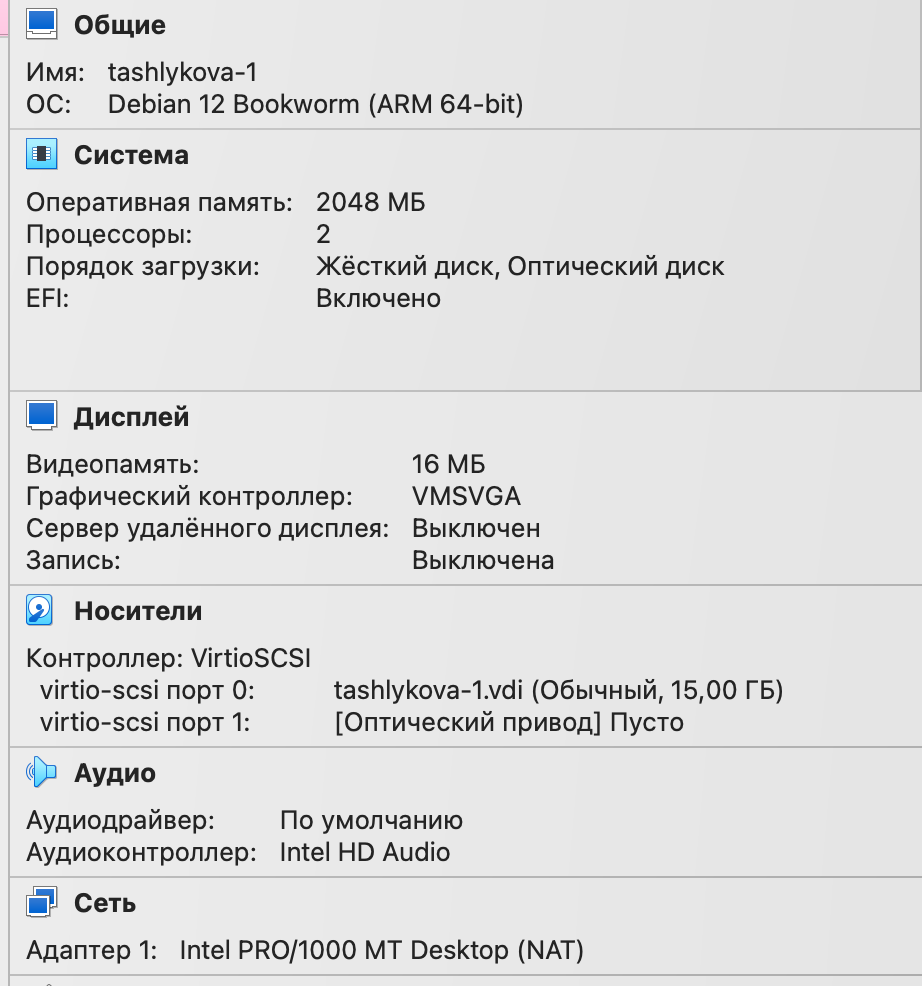
\includegraphics[height=10cm]{vm.png}
  \caption{\small Детали виртуальной машины}
\end{figure}

После загрузки системы на терминале tty1 отображается приглашение к вводу имени пользователя и пароля.
\begin{figure}[H]
  \centering
  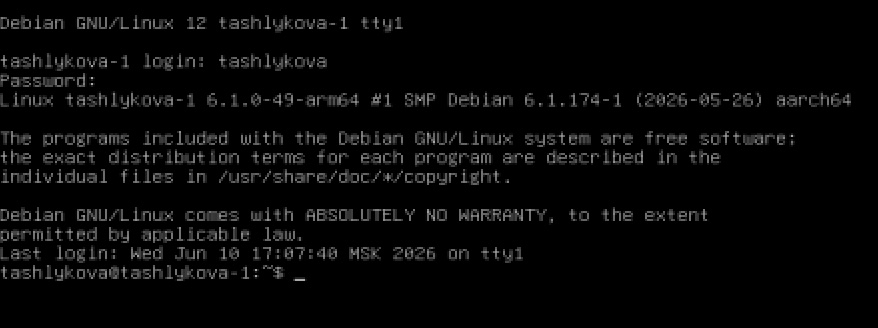
\includegraphics[height=5cm]{tty1.jpg}
  \caption{\small Приглашение tty1}
\end{figure}

Также в виртуальной машине была выполнена настройка проброса портов (Port Forwarding):
\begin{itemize}
    \item Тип подключения: NAT
    \item Протокол: TCP;
    \item Адрес хоста: 127.0.0.1;
    \item Порт хоста: 2222;
    \item Порт гостя: 22.
\end{itemize}
Это позволило подключаться к гостевой ОС через SSH.
\begin{figure}[h!]
  \centering
  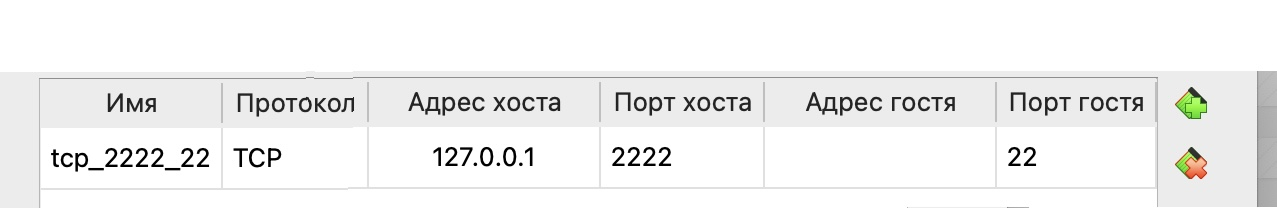
\includegraphics[height=2cm]{host.jpg}
  \caption{\small Проброс портов}
\end{figure}

Подключение к виртуальной машине выполнено с помощью встроенного SSH-клиента
Для беспарольной SSH-аутентификациии необходимо сгенерировать пару ключей, а публичный ключ скопировать на виртуальную машину.
\begin{verbatim}
ssh-keygen -t rsa -b 4096
ssh-copy-id -p 2222 tashlykova@127.0.0.1
ssh -p 2222 tashlykova@localhost 
\end{verbatim}
Благодаря этим действиям подключение к ВМ осуществляется без ввода пароля.

{\centering\subsection{Работа в командном интерпретаторе}}
Интерпретатор предоставляет большое количество команд для работы. С помощью $man$ я ознакомилась со справкой команд из списка задания, они приведены в таблице \ref{tab1}.
\begin{table}[H]
\centering
\renewcommand{\tablename}{\small{Таблица.}}
\caption{\small Основное назначение команд}
\label{tab1}
\begin{footnotesize}
    \begin{tabular}{|p{3cm}|p{7cm}|}
    \hline
    Команда & Пояснение \\
    \hline
    whoami & Вывод имени текущего пользователя\\ 
    \hline
    date & Вывод текущей даты и времени\\ 
    \hline
    uptime & Время работы системы и нагрузка\\ 
    \hline
    df & Информация о свободном месте на дисках\\ 
    \hline
    cp & Копирование файлов\\ 
    \hline
    mv & Перемещение/переименование файлов\\ 
    \hline
    touch & Создание пустого файла\\ 
    \hline
    rm & Удаление файлов\\ 
    \hline
    stat & Информация о файле (размер, права, время)\\ 
    \hline
    file & Определение типа файла\\ 
    \hline
    find & Поиск файлов по критериям\\ 
    \hline
    cat & Вывод содержимого файла\\ 
    \hline
    hexdump & Просмотр файла в шестнадцатеричном виде\\ 
    \hline
    less & Постраничный просмотр файла\\ 
    \hline
    time & Измерение времени выполнения команды\\
    \hline
    \end{tabular}
\end{footnotesize}
\end{table}

\begin{figure}[H]
  \centering
  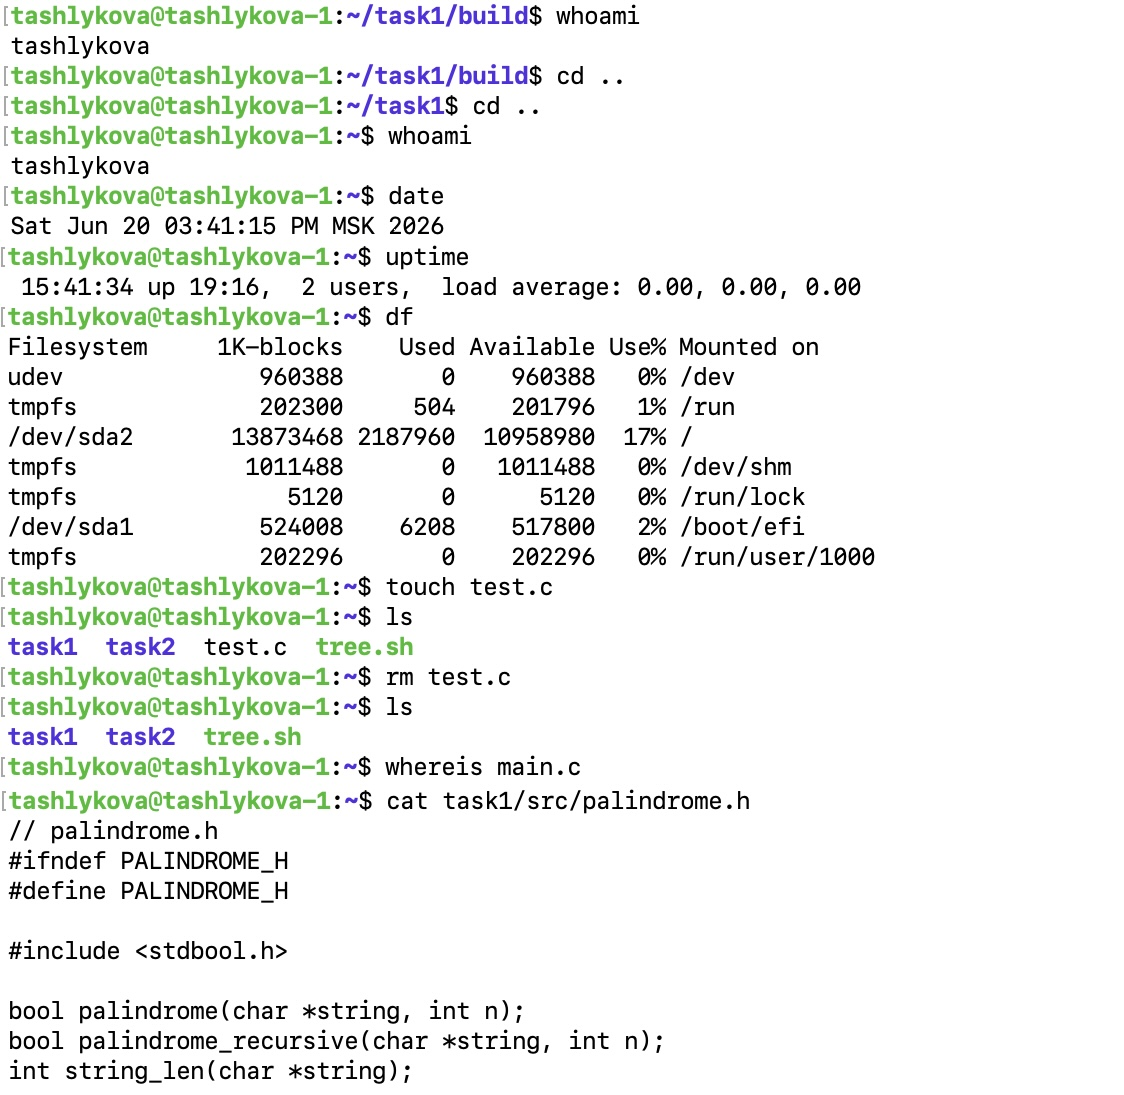
\includegraphics[height=15cm]{commands1.jpg}
  \caption{\small Работа в командном интерпретаторе}
\end{figure}

С помощью $history$ можно просмотреть всю истороию команд. Зафиксируем три последние:
\begin{verbatim}
chmod +x scripts/*.sh
./scripts/analyze_libs.sh 
./scripts/test_optimization.sh 
\end{verbatim}

Далее было необходимо исследовать зависимости между программой командного интерпретатора $/bin/bash$ и динамическими библиотеками операционной системы при помощи команды ldd. Для этого построим рекурсивное дерево зависимостей. Для наглядности был разработан скрипт $tree.sh$.

\begin{minted}[fontsize=\footnotesize]{c}
#tree.sh 
function print_deps() {
    local file=$1
    local indent=$2
    
    if [ ! -f "$file" ]; then
        echo "${indent}[НЕ НАЙДЕНО: $file]"
        return
    fi
    
    # Получаем зависимости через ldd
    ldd "$file" 2>/dev/null | grep "=> /" | awk '{print $3}' | while read lib; do
        echo "${indent}|__ $(basename $lib)"
        # Рекурсивно вызываем функцию с увеличенным отступом
        print_deps "$lib" "${indent}    "
    done
}
print_deps "$1" ""
\end{minted}

Все программы зависят от libc.so.6 -- стандартной библиотеки языка Си. Больше всего зависимостей у $bin/ls$.
\begin{figure}[H]
  \centering
  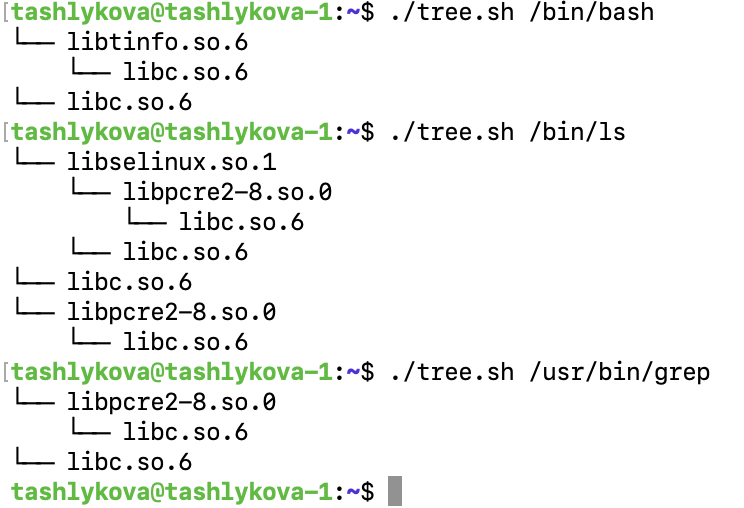
\includegraphics[height=8cm]{tree_ldd.png}
  \caption{\small Деревья зависимостей}
\end{figure}

{\centering\subsection{Разработка статических и динамических библиотек}}
В индивидуальном задании №1 было необходимо создать библиотеку с реализацией функции, которая проверяет является ли указанное слово палиндромом, при этом она должня быть реализована различными способами: с рекурсией и без рекурсии, также в реализации запрещалось использовать библиотечные функции.
Для этого я написала две основные функции $palindrome$, $palindrome\_recursive$ -- итеративная и рекурсивная реализация, а так же одну вспомогательную функцию $string\_len$, для вычисления длины строки.
\begin{minted}[fontsize=\footnotesize]{c}
#ifndef PALINDROME_H
#define PALINDROME_H

#include <stdbool.h>

bool palindrome(char *string, int n);
bool palindrome_recursive(char *string, int n);
int string_len(char *string);

#endif
\end{minted}

Алгоритм $palindrome$: сравниваются символы с начала и конца строки, постепенно сдвигаясь к центру. При обнаружении несовпадающей пары возвращается false. Время работы O(n/2), память O(1).\\
Алгоритм $palindrome\_recursive$: базовый случай -- пустая строка или строка из одного символа являются палиндромами. Иначе сравниваются первый и последний символы строки; при совпадении выполняется рекурсивный вызов для подстроки без крайних символов. Время работы O(n), память O(n).\\
Исходный код приведен в Приложении А.

Структура проекта:
\begin{verbatim}
task1
----CMakeLists.txt    
----src/
    |---CMakeLists.txt
    |---palindrome.c
    |---palindrome.h
----tests/
    |---CMakeLists.txt
    |---test_palindrome.c
    |---test_dlopen.c
----scripts/
    |---analyze_libs.sh
    |----test_optimization.sh
\end{verbatim}

Статическая библиотека -- это коллекция объектных файлов (.o), объединенных в один архивный файл. Во время компиляции программы, использующей статическую библиотеку, компоновщик (linker) копирует весь необходимый код из библиотеки в исполняемый файл. Таким образом, исполняемый файл становится самодостаточным и не зависит от наличия библиотеки в системе во время выполнения.

Динамическая (разделяемая) библиотека -- это коллекция скомпилированного кода, который загружается в память программы во время запуска. Исполняемый файл содержит только ссылки на функции и данные этой библиотеки, а не их копии. Это позволяет нескольким программам использовать одну и ту же копию библиотеки в памяти.

При обычной компоновке с динамической библиотекой, ОС автоматически загружает все необходимые библиотеки при запуске программы. Если какая-либо из них отсутствует, программа не запустится.

Однако существует еще более гибкий механизм работы с динамическими библиотеками -- их динамическая загрузка во время выполнения (runtime loading).
Runtime loading предоставляет программисту полный контроль над процессом, это означает, что программа может решить, какую библиотеку загрузить и какие функции из нее использовать, не на этапе компиляции, а уже в процессе своей работы.
Для реализации этого механизма в Unix/Linux используется набор функций, предоставляемых библиотекой dl (dynamic linking library)

Сборка библиотек происходит блягодаря сборочному файлу $src/CMakeLists.txt$.

{\centering\subsection{Исследование разделяемых библиотек}}
Как происходит тестирование функций $palindrome$ и $palindrome\_recursive$:
\begin{enumerate}
    \item Генерируются случайные строки заданной длины;

    \item Для каждой строки вычисляется длина с помощью $string\_len$;

    \item Выполняется проверка на палиндром (итеративная или рекурсивная);

    \item Измеряется процессорное время с помощью $clock()$;

    \item Результат усредняется по количеству итераций.
\end{enumerate}
Тестирование проходит для каждого типа линковки библиотеки.
Также дополнительно разработан скрипт для автоматического тестирования всех флагов оптимизации (O0, O1, O2, Os).



{\centering\subsection{Двоичные файлы и визуализация в псевдографике}}
Следующий этап научно-исследовательской работы -- разработка программы с использованием псевдографической библиотеки ncurses.

Ncurses («new curses») -- это библиотека предназначенная для управления вводом-выводом на терминал. Она позваляет работать с виртуальным экраном, создавать и управлять несколькими окнами на одном терминале, каждое со своим содержимым и атрибутами.

В рамках задания было неоходимо реализовать структуру с именем PRICE, содержащую следующие поля:
\begin{itemize}
    \item Название категории (строка Си).
    \item Название товара (строка Си).
    \item Стоимость товара в рублях (вещественный тип).
    \item Количество товаров в наличии (целочисленный тип).
\end{itemize}
А так же создать структуру описывающую заголовок базы данных:
\begin{itemize}
	\item Сигнатура формата файла (4 байта) – содержит первые 4 буквы фамилии латиницей.
	\item Номер транзакции (4 байта) – целое число, которое должно увеличиваться при каждом обращении к файлу, как при чтении, так и при записи.
	\item Количество структур в файле (4 байта) – количество структур данных из п.1 следующих за заголовком.
	\item Контрольная сумма (4 байта) – контрольная сумма всех данных следующих за заголовком по алгоритму CRC-32 вызываемая из библиотеки zlib.h
\end{itemize}

Далее представлена структура $PRICE$, а так же структура для заголовка базы данных $DB\_HEADER$.
\begin{minted}[fontsize=\footnotesize]{c}
typedef struct
{
    char *category;
    char *good;
    double price;
    unsigned int num;
} PRICE;

typedef struct 
{
    char signature[4];
    unsigned int tr_num;  
    unsigned int st_count;   
    unsigned int crc32;  
} DB_HEADER;
\end{minted}

% {\centering\subsection{}}

% {\centering\subsection{}}

{\centering\section{Результаты работы и эксперименты}}


{\centering\section*{Заключение}}\addcontentsline{toc}{section}{Заключение}

\newpage
\renewcommand{\bibname}{\vspace{-3.2cm}\centering\LargeСписок используемых источников}\addcontentsline{toc}{section}{Список используемых источников}
\begin{thebibliography}{8}

\bibitem{gametheory}
Петросян Л. А., Зенкевич Н. А., Семина Е. А. Теория игр : учеб. пособие для ун-тов. -- Москва : Высш. шк. : Книжный дом «Университет», 1998. - 304 с. - ISBN 5-06-001005-8.

\bibitem{virtualbox}
[Электронный ресурс] : 
\href{https://www.oracle.com/virtualization/virtualbox/}{https://www.oracle.com/virtualization/virtualbox/} 
(дата обращения: 22.05.2026).


\bibitem{devto_projects}
Adiati, A. <<Planning and Tracking Projects with GitHub's Projects Tool>> [Электронный ресурс] : 
\href{https://dev.to/adiatiayu/planning-and-tracking-projects-with-githubs-projects-tool-572l}{https://dev.to/adiatiayu/planning-and-tracking-projects-with-githubs-projects-tool-572l} 
(дата обращения: 23.05.2026).

\end{thebibliography}

\end{document}
